\chapter{Aplikacja internetowa}
\section{Architektura aplikacji} % (fold)
\label{sec:architektura_aplikacji}

\subsection{Wzorzec Model-Widok-Kontroler} % (fold)
\label{sub:wzorzec_model_widok_kontroler}
\paragraph{} % (fold)
\label{par:paragraph_name}
Model-Widok-Kontroler (\textit{ang. Model-View-Controller}) w skrócie MVC, jest wzorcem projektowym rozdzielający aplikację internetową na 3 warstwy : model, widok i kontroler, które komunikują się ze sobą wzajemnie (Rysunek \ref{fig:mvc-pic}). 

\subsubsection{Model}
\paragraph{}
Warstwa modelu odpowiada za reprezentację logiki systemu oraz dostęp do bazy danych. W projekcie za tę część aplikacji odpowiadają dwie biblioteki DLL : \textbf{PI.Service} oraz \textbf{PI.Data}.

\subsubsection{Widok}
\paragraph{}
Widok jest warstwą odpowiedzialną za wyświetlanie interfejsu użytkownika. Najczęściej widoki generowane są na podstawie modelu. W apliakcjach MVC widoki tylko wyświetlają informacje. Ta warstwa znajduje się w bibliotece \textbf{PI.Web}.

\subsubsection{Kontroler}
\paragraph{} 
Kontrolery to komponenty odpowiedzialne za utrzymanie interakcji z użytkownikiem, pracę z modelem i renderowaniem odpowiednich widoków. Kontrolery obsługują rządania użytkowników, konwertują parametry zapytań na modele i przekazują je do kolejnej warstwy. Kontrolery, podobnie jka widoki znajdują się w bibliotece \textbf{PI.Web}.  

\newpage
\begin{figure}[ht]
	\centering
		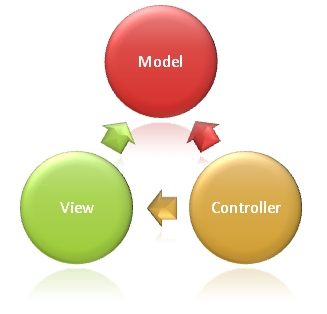
\includegraphics[width=0.5\linewidth]{assets/03_1.jpg}
	\caption{Schemat graficzny wzorca Model-Widok-Kontroler}
	\label{fig:mvc-pic}
\end{figure}

\subsection{Wzorzec Repozytorium} % (fold)
\label{sub:wzorzec_repozytorium}
\paragraph{} % (fold)
\label{par:}
\textit{Wzorzec Repozytorium} (\textit{Repository Pattern}) to popularna technika mająca na celu podział warstwy biznesowej na dwie części : \textit{Serwis} i \textit{Repozytorium}. \textit{Serwis} jest elementem odpowiedzialnym za logikę aplikacji oraz komunikację między kontrolerem, a repozytorium. \textit{Repozytorium} natomiast jest komponentem, ktorego zadanie polega na komunikacji z bazą danych : zapisywanie, pobieranie, edytowanie i usuwanie danych (model \textit{CRUD}). Takie rozsczepienie poszczególnych elementów pozwal na łatwe testowanie kodu, programowanie zorientowane na testy (\textit{ang. Test Driven Development}), szybką modernizację istniejącej logiki oraz rozbudowę aplikacji.

\paragraph{} % (fold)
\label{par:}
W projekcie \textit{Wzorzec Repozytorium} został zaimplementowany poprzez biblioteki \textbf{PI.Service (Serwis)} i \textbf{PI.Data (Repozytorium)}.
Dane z kontrolerów przekazywane są do \textit{Serwisu} pod postacią \textit{ViewModles} lub typów prymitywnych. \textbf{PI.Service} odpowiada za odpowiednią logikę przetwarzania danych, konwersji \textit{ViewModels} na \textit{Models} (przy wykorzystaniu narzędzia \textit{AutoMapper Sekcja \ref{sub:automapper}}) i przekazaniu ich do \textit{Repozytorium}.

\paragraph{} % (fold)
\label{par:}
Funkcją biblioteki \textbf{PI.Data} jest odbieranie danych z \textit{Serwisu} i dokonanie odpowiednich operacji bazodanowych przy użyciu \textit{EntityFramework (Sekcja \ref{sub:EntityFramework})}

\paragraph{} % (fold)
\label{par:}
Schemat działania logiki biznesowej w oparciu o \textit{Wzorzec Repozytorium} został przedstawiony na Rysunku \ref{fig:repository-pattern} .

\newpage
\begin{figure}[ht]
	\centering
		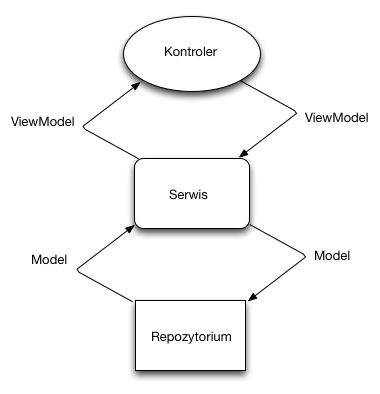
\includegraphics[width=0.5\linewidth]{assets/repository_pattern.png}
	\caption{Schemat przepływu danych przy wykorzystaniu Wzorca Repozytorium}
	\label{fig:repository-pattern}
\end{figure}

\subsection{Odwrócenie sterowania} % (fold)
\label{sub:odwr_cenie_sterowania}

% subsection odwr_cenie_sterowania (end)
% section architektura_aplikacji (end)

\section{Baza Danych} % (fold)
\label{sec:baza_danych}

% section baza_danych (end)

\section{Warstwa aplikacji} % (fold)
\label{sec:warstwa_aplikacji}

% section warstwa_aplikacji (end)

\section{Funkcjonalności} % (fold)
\label{sec:funkcjonalno_ci}

% section funkcjonalno_ci (end)